% Text for chapter 2
\chapter{The Physics of Coronal Loops}\label{ch:loops}

% Figure manager for Chapter 2
% spell-checker: disable
\begin{pycode}[chapter2]
name = 'chapter2'
ch2 = texfigure.Manager(
    pytex,
    os.path.join('.', name),
    number=2,
    **{k: os.path.join('.', name, v) for k,v in manager_opts.items()}
)
import tempfile
import shutil

from hydrad_tools.configure import Configure
from hydrad_tools.parse import Profile, Strand
from synthesizAR.physics import RTVScalingLaws

from physics import power_law_rad_loss, isothermal_loop, beta_gary
\end{pycode}
% spell-checker: enable

% conceptual comments on loops, see Reale (2010)
% define plasma beta
% define distinction between loops and strands

% spell-checker: disable %
\begin{pycode}[chapter2]
fig = plt.figure(figsize=texfigure.figsize(
    pytex,
    scale=1,
    height_ratio=2/3,
))

# Beta versus height
h = np.logspace(-2, 4, 1000) * u.Mm
beta_s = beta_gary(h, 'sunspot')
beta_p = beta_gary(h, 'plage')
ax1 = plt.subplot2grid((1,3),(0,0),)
ax1.plot(beta_s, h, label='sunspot', color=PALETTE[0])
ax1.plot(beta_p, h, label='plage', color=PALETTE[1])
ax1.axvline(x=1, ls='--', color='k')
ax1.axhline(y=(250*u.km).to(u.Mm).value, ls=':', color='k')
ax1.axhline(y=(2500*u.km).to(u.Mm).value, ls=':', color='k')
ax1.axhline(y=(2*const.R_sun).to(u.Mm).value, ls=':', color='k')
ax1.set_xscale('log')
ax1.set_yscale('log')
ax1.set_xlim(6e-6,2e2)
ax1.set_ylim(1e-2,1e4)
ax1.set_xlabel(r'$\beta$')
ax1.set_ylabel(r'$h$ $[\si{\mega\m}]$')
ax1.legend(loc='lower left', frameon=False)

# TRACE Map
m = Map(os.path.join(ch2.data_dir, 'trace_example.fits'))
m = Map(m.data, {**m.meta, 'wavelnth': m.meta['wave_len']},)
m = m.submap(
    SkyCoord(Tx=-1150*u.arcsec,Ty=100*u.arcsec,frame=m.coordinate_frame),
    SkyCoord(Tx=-850*u.arcsec,Ty=400*u.arcsec,frame=m.coordinate_frame),
)
ax2 = plt.subplot2grid((1,3),(0,1),colspan=2,projection=m)
m.plot(axes=ax2,
       annotate=False,
       norm=ImageNormalize(
           vmin=max(0,m.data.min()),
           vmax=m.data.max(),stretch=AsinhStretch(0.005)),
)
ax2.grid(alpha=0)
lon,lat = ax2.coords[0],ax2.coords[1]
lon.set_ticks_visible(False)
lat.set_ticks_visible(False)
lon.set_ticklabel_visible(False)
lat.set_ticklabel_visible(False)
plt.subplots_adjust(wspace=0.1)

# Save
tfig = ch2.save_figure('beta-trace', fext='.pdf')
tfig.caption = r'\textit{Left:} A simple empirical model of $\beta$ as a function of height, $h$, above the solar surface as calculated by Equation 2 and Equation 3 of \citet{gary_plasma_2001} for the magnetic field above a sunspot (blue) and a plage region (orange). The dotted lines indicate the tops of the photosphere, chromosphere and corona. The dashed line denotes $\beta=1$. Adapted from Figure 3 of \citet{gary_plasma_2001}. \textit{Right:} An arcade of loops extending into the corona observed off the solar limb by the TRACE satellite on 6 November 1999. Adapted from Figure 11 of \citet{reale_coronal_2010}.'
\end{pycode}
\py[chapter2]|tfig|
% spell-checker: enable %

\section{Hydrostatics}\label{sec:hydrostatic}

\subsection{Equations of Hydrostatic Equilibrium}\label{sec:hydrostatic_equations}

For a single strand in hydrostatic equilibrium with uniform cross-sectional area, the equations of pressure and energy balance as a function of $s$, the coordinate parallel to the magnetic field, are given by,
\begin{align}
    Q &= n^2\Lambda(T) + \frac{d}{ds}F_c, \label{eq:hydrostatic_energy} \\
    \frac{d}{ds}p &= m_ing, \label{eq:hydrostatic_pressure} \\
    p &= 2k_BnT, \label{eq:ideal_gas_law}
\end{align}
where $Q$ is the heating rate, $\Lambda(T)$ is the radiative loss term, $F_c$ is the conductive flux, $p$ is the thermal pressure, $n$ is the number density, $T$ is the temperature, $m_i$ is the average ion mass, $g=-g_\solar\left(\frac{R_\solar}{r}\right)^2\frac{dr}{ds}$ is the gravitational acceleration along the fieldline, $r$ is the radial distance from the center of the Sun, and $g_\solar$ is the gravitational acceleration at the solar surface ($r=R_\solar$).

To determine $n$ and $T$ as a function of $s$ along the strand, one must solve \autoref{eq:hydrostatic_energy} and \autoref{eq:hydrostatic_pressure} given some predefined heating rate $Q$, which is, in general, a function of the loop coordinate and is often assumed to be proportional to powers of $n$ and $T$ \citep{priest_magnetohydrodynamics_2014}. Both of these equations are subject to closure by the equation of state given in \autoref{eq:ideal_gas_law}.

\autoref{eq:hydrostatic_pressure} says that the downward gravitational pull on the plasma is balanced by the gradient of the thermal pressure. \autoref{eq:hydrostatic_energy} says that the energy lost by radiation and thermal conduction in the corona must be balanced by coronal heating. I will now discuss the conductive flux and radiative loss terms in more detail. Several possible solution methods for \autoref{eq:hydrostatic_energy} and \autoref{eq:hydrostatic_pressure} are discussed in \autoref{sec:isothermal}, \ref{sec:scaling_laws}, and \ref{sec:hydrostatic_numerical}.

\subsubsection{Conductive Flux Term}\label{sec:heat-flux}

Thermal conduction efficiently transfers energy from regions of high temperature to regions of low temperature in the direction parallel to the magnetic field and opposite to the temperature gradient. However, cross-field (i.e. perpendicular to the magnetic field) thermal conduction is severely inhibited due to the low-$\beta$ nature of the corona such that energy transfer is limited to the field-aligned direction. 

It is commonly assumed that the field-aligned thermal conduction, $F_c$, is well-described by expression of \citet{spitzer_transport_1953},
\begin{equation}\label{eq:spitzer-harm}
    F_c = -\kappa_0 T^{5/2} \frac{dT}{ds},
\end{equation}
where $\kappa_0\sim\SI{e-6}{\erg\per\cm\per\second\per\kelvin\tothe{7/2}}$ is the coefficient of thermal conduction in the field-aligned direction. In the corona, thermal conduction is an energy sink needed to balance coronal heating. However, in the TR, where $Q=0$, thermal conduction is an energy source to compensate for losses due to radiation. Thus, $F_c$ be used to define the boundary between the TR and the corona such that the base of the corona is the point at which thermal conduction transitions from an energy source to a sink \citep{vesecky_numerical_1979,bradshaw_new_2010}. Note that no energy is lost from the system due to the heat flux; it is only a mechanism for transferring energy between the corona and transition region provided the conductive flux to the cooler, underlying chromosphere is negligible such that the loop is thermally isolated.  

According to \autoref{eq:spitzer-harm}, $F_c\to\infty$ as $\frac{dT}{ds}\to\infty$. However, at low densities, there may be an insufficient number of particles to support the implied heat flux such that the heat flux saturates at the \textit{free-streaming limit} \citep{patsourakos_coronal_2005,bradshaw_explosive_2006,bradshaw_collisional_2013}. Failure to account for this limiting of the heat flux can result in overestimation of the cooling due to thermal conduction, particularly in cases where the heating is very impulsive. A more detailed discussion of the free-streaming limit is given in \autoref{hot-plasma:subsec:hf_theory}.

In a rarified, impulsively heated plasma, the electron mean free path may become large relative to the temperature length scale of the plasma such that the electron distribution becomes non-Maxwellian \citep{bradshaw_collisional_2013}. In this case, non-local contributions to the heat flux may become important such that determining the heat flux at any one point along the loop requires integrating over the entire loop. This ``non-localization'' of the heat flux has been addressed by a number of authors \citep{ljepojevic_heat_1989,karpen_nonlocal_1987,luciani_nonlocal_1983,west_lifetime_2008} and is likely to have important consequences for the observability of hot, low-density plasmas.

\subsubsection{Radiative Loss Term}\label{sec:rad-loss}

Energy from the coronal plasma is also lost to space by radiation. The radiative loss term is proportional to $n^2$ so it is most dominant in areas where the density is high. The amount of energy which the plasma radiates away by spectral line and continuum emission also depends on the temperature through the radiative loss function, $\Lambda(T)$, given by,
\begin{equation}\label{eq:rad-loss}
    \Lambda(T) = \sum_{X,k}\left(\sum_{\{ji\}}4\pi G_{ji}  + \int_0^\infty\dd{\lambda}P_{X,k}^\textup{cont.} \right),
\end{equation}
where $G_{ji}$ is the contribution function of transition $ji$ in ion $k$ of element $X$ as given by \autoref{eq:contribution_function}, $P_{X,k}^\textup{cont.}$ is the total continuum emissivity of ion $k$ in element $X$ (see \autoref{sec:continuum}), and $\{ji\}$ is the set of all atomic transitions in ion $k$ of element $X$. Practically speaking, the summations are taken over all elements, ions, and transitions in the CHIANTI atomic database (see \autoref{sec:chianti}). Note that $\Lambda(T)$ is also dependent on the density due to the density dependence of $G_{ji}$ though this dependence is relatively weak compared to that of $T$.

% spell-checker: disable %
\begin{pycode}[chapter2]
with h5py.File(os.path.join(ch2.data_dir, 'chianti_rad_loss.h5'), 'r') as hf:
    T = u.Quantity(hf['temperature'], hf['temperature'].attrs['unit'])
    Lambda = u.Quantity(hf['radiative_loss'], hf['radiative_loss'].attrs['unit'])
fig = plt.figure(figsize=texfigure.figsize(
    pytex,
    scale=0.85,
    height_ratio=0.75,
    figure_width_context='figurewidth',
))
ax = fig.gca()
ax.plot(T, Lambda, color=PALETTE[0], label='CHIANTI')
ax.plot(T, power_law_rad_loss(T, kind='klimchuk'), color=PALETTE[1], label='RK')
ax.plot(T, power_law_rad_loss(T, kind='rtv'), color=PALETTE[2], label='RTV')
ax.set_xscale('log')
ax.set_yscale('log')
ax.set_xlim(T[[0,-1]].value)
ax.set_ylim(5e-24,1e-21)
ax.set_xlabel(r'$T$ $[\si{\kelvin}]$')
ax.set_ylabel(r'$\Lambda$ $[\si{\erg\cubic\cm\per\second}]$')
ax.legend(loc=1, frameon=False)
tfig = ch2.save_figure('radiative-loss', fext='.pgf')
tfig.caption = r'Radiative loss as a function of temperature for an optically thin plasma. The blue line shows the true value of $\Lambda$ computed by CHIANTI using the abundances of \citet{feldman_potential_1992} and assuming a constant density of \SI{e9}{\per\cubic\cm}. The orange line shows the Raymond-Klimchuk (RK) power-law approximation given in \citet{klimchuk_highly_2008} and the green line shows the power-law approximation of \citet[RTV]{rosner_dynamics_1978}.'
tfig.figure_width = r'0.85\textwidth'
\end{pycode}
\py[chapter2]|tfig|
% spell-checker: enable %

Calculating $\Lambda(T)$ can be computationally expensive as it requires solving \autoref{eq:level_pop}, the level population equation, for each ion over a large temperature range. \citet{rosner_dynamics_1978} calculate an analytic fit to the radiative loss function of the form,
\begin{equation}\label{eq:rad-loss-power-law}
    \Lambda(T) = \chi T^\alpha,
\end{equation}
where $\chi$ and $\alpha$ are piecewise functions in $T$. The values of $\alpha$ and $\chi$ are given in Appendix A of \citet{rosner_dynamics_1978}. \citet{klimchuk_highly_2008} provide an improved piecewise fit to $\Lambda(T)$ of the same form as \autoref{eq:rad-loss-power-law} using updated atomic radiative loss calculations. Additionally, \citet{cargill_active_2014} provide a minor fix to the fits of \citet{klimchuk_highly_2008} given the results of \citet{reale_role_2012} who find that using the power-law fit of \citet{rosner_dynamics_1978} versus the full CHIANTI radiative loss function gives significantly different cooling behavior in an impulsively heated loop. \autoref{fig:radiative-loss} shows a comparison between the full radiative loss function as computed by \autoref{eq:rad-loss} (blue) and the power-law approximations of \citet[orange]{klimchuk_highly_2008} and \citet[green]{rosner_dynamics_1978}. 

\subsection{The Isothermal Limit}\label{sec:isothermal}

I now discuss several methods for solving the hydrostatic energy and pressure equations. First, consider the case of an isothermal, semi-circular loop where $T(s)=T$ such that $dT/ds=0$ and $F_c=0$ in the case where heat flux, $F_c$, is given by \autoref{eq:spitzer-harm}. \autoref{eq:hydrostatic_energy} and \autoref{eq:hydrostatic_pressure} then become,
\begin{align}
Q &= n^2\Lambda(T), \\
\frac{d}{ds}p &= -p\frac{m_ig_\solar}{2k_BT}\frac{R_\solar^2}{r^2(s)}\cos{\left(\frac{\pi s}{2L}\right)},
\end{align}
where $r(s) = R_\solar + \frac{2L}{\pi}\sin{\left(\frac{\pi s}{2L}\right)}$ and $L$ is the half-length of the loop. Note that in this case, the heating term is now balanced only by the radiative loss term. 

Defining the hydrostatic scale height as $\lambda_h=2k_BT/m_ig_\solar$, making a change of variables $\xi=r(s)$ such that $d\xi=\cos{(\pi s / 2L)}ds$, and separating variables, the pressure equation becomes,
\begin{align}
    \int_{p_0}^p\dd{p^\prime}\frac{1}{p^\prime} &= -\frac{R_\solar^2}{\lambda_h}\int_{R_\solar}^\xi\dd{\xi^\prime}\frac{1}{\xi^{\prime2}},\nonumber \\
    \ln\left(\frac{p}{p_0}\right) &= \frac{R_\solar^2}{\lambda_h}\left(\frac{1}{\xi} - \frac{1}{R_\solar}\right),\nonumber \\
    p(s) &= p_0\exp{\left[-\frac{1}{\lambda_h}\frac{(2L/\pi)\sin{(\pi s/2L)}}{1 + (2L/\pi R_\solar)\sin{(\pi s/2L)}}\right]}, \label{eq:isothermal_pressure}
\end{align}
where $p_0$ is the pressure at $s=0$. At the apex of the loop, $s=L$, the pressure is,
\begin{equation*}
    p(L) = p_0\exp{\left[-\frac{2L/\pi}{\lambda_h(1 + 2L/\pi R_\solar)}\right]}.
\end{equation*}

% spell-checker: disable %
\begin{pycode}[chapter2]
fig = plt.figure(figsize=texfigure.figsize(pytex, scale=1,))
ax = fig.gca()

temps = u.Quantity([1e5, 5e5, 1e6, 2e6, 5e6],'K')
s = np.linspace(0, 500, 100)*u.Mm
n0 = 1e10 * u.cm**(-3)

for i,t in enumerate(temps):
    n_v,_,_ = isothermal_loop(s, t, n0,vertical=True)
    n_c,_,_ = isothermal_loop(s, t, n0,vertical=False)
    ax.plot(s, n_v, color=f'C{i}', ls='--')
    ax.plot(s, n_c, color=f'C{i}', ls='-',
            label=r'\SI{{{:1.0g}}}{{\kelvin}}'.format(t.to(u.K).value))

ax.set_xlim(s[[0,-1]].value)
ax.set_ylim(1e6, n0.value)
ax.set_yscale('log')
ax.set_xlabel(r'$s$ $[\si{\mega\m}]$')
ax.set_ylabel(r'$n$ $[\si{\per\cubic\cm}]$')
ax.legend(frameon=False, loc='lower center',ncol=2)

tfig = ch2.save_figure('isothermal-loop', fext='.pgf')
tfig.caption = r'Density as a function of field-aligned coordinate, $s$, for an isothermal flux tube assuming a vertical (dashed) and semi-circular (solid) geometry for a half length of $L=\SI{500}{\mega\m}$ and a footpoint density of $n_0=\SI{e10}{\per\cubic\cm}$. The different colors correspond to different temperatures, $T$, as denoted in the legend.'
\end{pycode}
\py[chapter2]|tfig|
% spell-checker: enable %

In the limit of a vertical flux tube such that the loop has no curvature, \autoref{eq:isothermal_pressure} becomes,
\begin{equation}\label{eq:isothermal_pressure_vertical}
    p(s) = p_0\exp{\left[-\frac{s}{\lambda_h(1 + s/R_\solar)}\right]} = p_0\exp{\left[-\frac{h}{\lambda_p}\right]},
\end{equation}
where $\lambda_p=\lambda_h(1 + h/R_\solar)$ is the pressure scale height. Similarly, from \autoref{eq:ideal_gas_law}, the density can be expressed as,
\begin{equation*}
    n(s) = n_0\exp{\left[-\frac{h}{\lambda_p}\right]},
\end{equation*} 
where $n_0=p_0/2k_BT$. Thus, in a vertical, gravitationally stratified flux tube, the pressure and density fall of exponentially with a scale height $\lambda_p$. For short loops ($h\ll R_\solar$), gravitational stratification plays only a minor role in the pressure (and density) structure and $\lambda_p\approx\lambda_h$. In the case of longer loops, gravitational stratification becomes more important. Additionally, note that $\lambda_h\propto T$ such that hotter loops are less stratified. \autoref{fig:isothermal-loop} shows the density as a function of $s$ for a vertical flux tube and half of a semi-circular flux tube for a range of temperatures. As the temperature increases, the gravitational stratification of the density decreases such that hot plasma is likely to be found at higher altitudes while cooler plasma is more likely to be found near the base of the loop.

Continuing with the assumption of a vertical flux tube, the heating term can now be expressed as,
\begin{equation}
    Q = n_0^2 \Lambda(T) \exp{\left(-\frac{h}{\lambda_p/2}\right)}.
\end{equation}
Note that the heating falls off twice as fast as the pressure such that in long loops, the heating needed to balance losses from radiation will be concentrated near the footpoints.

\subsection{Scaling Laws}\label{sec:scaling_laws}

%RTV, Serio, Martens (2 paragraphs)

In the non-isothermal case, an analytic solution of \autoref{eq:hydrostatic_energy} and \autoref{eq:hydrostatic_pressure} is not possible due to the $dF_c/ds$ term being nonlinear in $T$. As a result, a number of so-called scaling laws have been developed to provide analytic and interpretable approximations for the thermal structure of coronal loops. In order to interpret early space-based coronal observations made with the S-054 \textit{SkyLab} X-ray telescope, \citet{rosner_dynamics_1978} derived two scaling laws relating the heating and maximum temperature to the isobaric pressure and loop length. I will now summarize this derivation.

Using \autoref{eq:ideal_gas_law} and \autoref{eq:spitzer-harm}, \autoref{eq:hydrostatic_energy} can be written as,
\begin{equation*}
    \frac{F_c}{\kappa_0T^{5/2}}\frac{dFc}{dT} = \frac{p^2}{4k_B^2T^2} - Q.
\end{equation*}
Separating variables and integrating from the base of the loop yields,
\begin{equation*}
    \int_{F_{c,0}}^{F_c}\dd{F_c^\prime}F_c^\prime = \frac{\kappa_0 p^2}{4k_B^2}\int_{T_0}^T\dd{T^\prime}T^{\prime 1/2}\Lambda(T^\prime) - \kappa_0\int_{T_0}^T\dd{T^\prime}T^{\prime 5/2}Q,
\end{equation*}
where the ``0'' subscript denotes a quantity at the base of the loop. If the loop is thermally isolated from the lower atmosphere, $F_{c,0}=0$ such that no thermal energy is conducted across the lower boundary. Using this assumption to simplify the left-hand side gives,
\begin{equation}\label{eq:rtv:fc2}
    F_c^2 = f_R(T) - f_H(T),
\end{equation}
where,
\begin{align}
    f_R(T) &= \frac{\kappa_0p^2}{2k_B^2}\int_{T_0}^T\dd{T^\prime}T^{\prime 1/2}\Lambda(T^\prime), \label{eq:rtv:fr_integral} \\
    f_H(T) &= 2\kappa_0\int_{T_0}^T\dd{T^\prime}T^{\prime 5/2}Q. \label{eq:rtv:fh_integral}
\end{align}
Note that \autoref{eq:rtv:fc2} requires that $f_R(T)\ge f_H(T)$ to guarantee a physical solution for the heat flux. Using the definition of the classical heat flux, \autoref{eq:spitzer-harm}, again and integrating once more from the base of the loop yields,
\begin{align}
    \left(\kappa_0T^{5/2}\frac{dT}{ds}\right)^2 &= f_R(T) - f_H(T), \nonumber \\
    \kappa_0T^{5/2}\frac{dT}{ds} &= (f_R(T) - f_H(T))^{1/2}, \nonumber \\
    s - s_0 &= \kappa_0\int_{T_0}^T\dd{T^\prime}\frac{T^{\prime 5/2}}{\sqrt{f_R(T^\prime) - f_H(T^\prime)}} \label{eq:rtv:fr_fh_integral},
\end{align}
where $s=s(T_0)$ is the coordinate at the base of the loop. Using the appropriate boundary conditions, \autoref{eq:rtv:fr_fh_integral} can then be used to derive both scaling laws.

First, \autoref{eq:rtv:fr_integral} can be simplified by using piecewise power-law approximation in \autoref{eq:rad-loss-power-law}. For $T>\SI{e5}{\kelvin}$, $\alpha=-1/2$ is a suitable approximation \citep[see Appendix A of][]{rosner_dynamics_1978} and assuming $T\gg T_0$, \autoref{eq:rtv:fr_integral} becomes
\begin{equation}\label{eq:rtv:fr}
    f_R(T) = \frac{\kappa_0\chi_0 p^2}{2k_B^2}T,
\end{equation}
where $\chi_0=\SI{e-18.8}{\erg\cm\cubed\kelvin\tothe{1/2}\per\second}$.

% spell-checker: disable %
\begin{pycode}[chapter2]
p0 = np.logspace(-2,3,100) * u.dyne/(u.cm**2)
loop_lengths = u.Quantity([1e9,1e10,1e11], 'cm')

fig = plt.figure(figsize=texfigure.figsize(pytex, scale=1,))
ax = fig.gca()

# Plot pressure versus in temperature
for i,L in enumerate(loop_lengths):
    rtv = RTVScalingLaws(L, pressure=p0)
    ax.plot(p0, rtv.max_temperature, color=PALETTE[i],
            label=r'$L=\SI{{{:.0f}}}{{\mega\m}}$'.format(L.to(u.Mm).value))

# Ticks and labels
ax.set_xscale('log')
ax.set_yscale('log')
ax.set_xlabel(r'$p$ $[\si{\dyne\per\square\cm}]$')
ax.set_ylabel(r'$T_\textup{max}$ $[\si{\kelvin}]$')
ax.set_xlim(p0[[0,-1]].value)
ax.set_ylim(1e6, 1e8)
ax.legend(frameon=False, loc=2)

# Save
tfig = ch2.save_figure('rtv-tmax', fext='.pgf')
tfig.caption = r'Loop apex temperature, $T_\textup{max}$, as a function of pressure, $p$, calculated from \autoref{eq:rtv:scaling-law-tmax} for several different values of the loop half-length, $L$. Adapted from Figure 9 of \citet{rosner_dynamics_1978}.'
\end{pycode}
\py[chapter2]|tfig|
% spell-checker: enable %

At the base of the loop, losses due to radiation dominate over energy supplied by the heating term such that $f_R(T) \gg f_H(T)$. Using this condition and \autoref{eq:rtv:fr} and integrating the right-hand side of \autoref{eq:rtv:fr_fh_integral} from the base of the loop ($T_0$) to the apex ($T_\textup{max}$), \autoref{eq:rtv:fr_fh_integral} becomes,
\begin{align}
    s_\textup{max} - s_0 = \frac{k_B}{p}\sqrt{\frac{2\kappa_0}{\chi_0}}\int_{T_0}^{T_\textup{max}}\dd{T^\prime}T^{\prime 2}, \nonumber \\
    s_\textup{max} - s_0 = \frac{k_B}{3p}\sqrt{\frac{2\kappa_0}{\chi_0}}(T_\textup{max}^3 - T_0^3), \nonumber
\end{align}
where $s_\textup{max}=s(T_\textup{max})$ is the coordinate at the apex of the loop where the temeperature is maximized. Defining the loop half-length, the distance between the apex and the base, as $L=s(T_\textup{max}) - s(T_0)$, assuming $T_\textup{max}\gg T_0$ since $T$ monotonically increases from the base to the apex, and solving for $T_\textup{max}$ yields the first scaling law,
\begin{equation}\label{eq:rtv:scaling-law-tmax}
    T_\textup{max} = c_1(pL)^{1/3},
\end{equation}
where $c_1=\left(\frac{3}{k_B}\sqrt{\frac{\chi_0\kappa_0}{2}}\right)^{1/3}\approx\py[chapter2]|f'{rtv.c1.to(u.K*(u.cm/u.dyne)**(1/3)).value:.0f}'|\,\si{\kelvin\cm\tothe{1/3}\per\dyne\tothe{1/3}}$. \autoref{fig:rtv-tmax} shows the apex temperature, $T_\textup{max}$, as a function of $p$ for several different loop half-lengths. Note that longer loops have higher apex temperatures.

If the loop is heated uniformly, the maximum temperature will occur at the apex such that $dT/ds=0$ at $s=s_\textup{max}$ and by \autoref{eq:spitzer-harm}, the heat flux at the apex also vanishes. In this case, plugging \autoref{eq:rtv:fh_integral} and \autoref{eq:rtv:fr} into \autoref{eq:rtv:fc2} gives,
\begin{align}
    f_R(T_\textup{max}) &= f_H(T_\textup{max}), \nonumber \\
    \frac{\kappa_0\chi_0}{2k_B^2}p^2T_\textup{max} &= 2\kappa_0Q\int_{T_0}^{T_\textup{max}}\dd{T} T^{5/2}, \nonumber \\
    \frac{\chi_0}{2k_B^2}p^2T_\textup{max} &= \frac{4}{7}Q(T_\textup{max}^{7/2} - T_0^{7/2}).
\end{align}
Using the approximation $T_\textup{max}\gg T_0$, the second term on the right-hand side can be dropped. Finally, using the first scaling law (\autoref{eq:rtv:scaling-law-tmax}) and solving for $Q$ gives the second scaling law of \citet{rosner_dynamics_1978},
\begin{equation}\label{eq:rtv:scaling-law-heat}
    Q = c_2 p^{7/6}L^{-5/6},
\end{equation}
where $c_2=\frac{7\chi_0}{8k_B^2}c_1^{-5/2}\approx\py[chapter2]|f'{rtv.c2.to(u.erg**(-1/6)*u.cm**(4/3)/u.s).value:.0f}'|\,\si{\cm\tothe{4/3}\per\erg\tothe{1/6}\per\second}$. Note that this scaling law implies that less heat is needed to sustain a long loop compared to a short loop at the same pressure.

\citet{serio_dynamics_1991} extend the work of \citet{rosner_dynamics_1978} by considering two additional cases: (1) loops with $L$ greater than th pressure scale height such that the isobaric approximation does not hold; and (2) loops with a local temperature minimum at the top. They considered a more general form of the heating function, $Q(s)=Q_0\exp{(-s/\lambda_H)}$, where the heating is now stratified and falls off exponentially over a heating scale height $\lambda_H$. The modified scaling laws of \citet{serio_dynamics_1991} are,
\begin{align}
    T_\textup{max} &= c_1(p_0L)^{1/3}\exp{\left[-0.04L\left(\frac{2}{\lambda_H} + \frac{1}{\lambda_p}\right)\right]}, \label{eq:serio:scaling-law-tmax} \\
    Q_0 &= c_2p_0^{7/6}L^{-5/6}\exp{\left[0.5L\left(\frac{1}{\lambda_H} - \frac{1}{\lambda_p}\right)\right]}, \label{eq:serio:scaling-law-heat}
\end{align}
where $p_0$ is the pressure at the base of the loop, $Q_0$ is the heating rate at the base of the loop, $\lambda_p$ is the pressure scale height as defined in \autoref{sec:isothermal}. The derivation is largely the same as that of \citet{rosner_dynamics_1978} except that $p$ is allowed to vary with $s$ according to \autoref{eq:isothermal_pressure_vertical} in the limit of no gravitational stratification. Note that the scaling laws of \citet{rosner_dynamics_1978} (\autoref{eq:rtv:scaling-law-tmax} and \autoref{eq:rtv:scaling-law-heat}) are recovered in the limits of constant pressure ($\lambda_p\to\infty$) and uniform heating ($\lambda_H\to\infty$). If the heating is sufficiently stratified such that $\lambda_H<L/2$, there will be local temperature minimum at the apex. In cases where the heating is very localized near the footpoints such that $\lambda_H<\lambda_p/3$, a cool condensation may form at the apex, causing the loop to be Rayleigh-Taylor unstable. See \autoref{sec:tne} for additional discussion of non-equilibrium in steadily-heated loops.

More recently, \citet{martens_scaling_2010} derived an analytic expression for the temperature profile along the loop under the assumption of constant pressure $p_0$ and using a heating function of the form,
\begin{equation}\label{eq:martens:heating}
    Q = C_Qp_0^{\beta^\star}T^{\alpha^\star}, 
\end{equation}
where $C_Q$ is a constant of proportionality and $\beta^\star$ and $\alpha^\star$ determine the dependence of $Q$ on $p_0$ and $T$, respectively. Assuming a radiative loss function of the form of \autoref{eq:rad-loss-power-law}, \citeauthor{martens_scaling_2010} solve a dimensionless form of \autoref{eq:hydrostatic_energy} and find a closed-form expression for the temperature as a function of the field-aligned coordinate, $s$,
\begin{equation}\label{eq:martens:temperature}
    T(s) = T_\textup{max}\left[\beta_r^{-1}(s/L;\lambda+1,1/2)\right],
\end{equation}
where $\beta_r^{-1}$ is the inverse of the regularized incomplete $\beta$-function \citep[see Section 6.6 of][]{abramowitz_handbook_1972}, $\lambda=\frac{11/2+\gamma}{2(2 + \gamma + \alpha^\star)} - 1$, and $\gamma = -\alpha$ from \autoref{eq:rad-loss-power-law}.

\citet{martens_scaling_2010} points out that the solution in \autoref{eq:martens:temperature} is overconstrained by the boundary conditions on his dimensionless energy equation such that \autoref{eq:martens:temperature} is only valid for specific sets of parameters. These additional constraints produce two scaling laws of similar form to those of \citet{rosner_dynamics_1978,serio_dynamics_1991}. The scaling laws of \citet{martens_scaling_2010} are,
\begin{align}
    p_0L &= T_\textup{max}^{\frac{11+2\gamma}{4}} \left(\frac{\kappa_0}{\chi_0^\prime}\right)^{1/2}\frac{(3-2\gamma)^{1/2}}{4 + 2\gamma + 2\alpha^\star} B(\lambda + 1, 1/2), \label{eq:martens:scaling_law_tmax} \\
    Q_\textup{apex} &= \frac{p_0^2\chi_0(7/2 + \alpha^\star)}{T_\textup{max}^{(2+\gamma)}(3/2 - \gamma)}, \label{eq:martens:scaling_law_heating}
\end{align}
where $B$ is the complete $\beta$-function \citep[see Equation 6.2.1 of][]{abramowitz_handbook_1972}, $\chi_0^\prime=\chi_0/4k_B^2$, and $Q_\textup{apex}$ is the heating rate at the apex of the loop (i.e. where $T=T_\textup{max}$). \autoref{eq:martens:scaling_law_tmax} and \autoref{eq:martens:scaling_law_heating} provide a generalization of the scaling laws of \citet{rosner_dynamics_1978} for non-uniform heating along the loop. Notice that in the case of uniform heating ($\alpha^\star=0$) and $\gamma=-\alpha=1/2$, \autoref{eq:martens:scaling_law_tmax} and \autoref{eq:martens:scaling_law_heating} reduce to \autoref{eq:rtv:scaling-law-tmax} and \autoref{eq:rtv:scaling-law-heat}, respectively. In \autoref{ch:synthesizar}, I use the scaling laws of \citet{martens_scaling_2010} to efficiently model time-independent emission from an \AR{} composed of many hundreds of loops.  

\subsection{Numerical Solutions}\label{sec:hydrostatic_numerical}

%Show basic hydrostatic solutions via shooting method (1 paragraph)

While the analytical expressions outlined in \autoref{sec:scaling_laws} provide useful approximations of the thermal structure of a coronal loop, it is often necessary to solve the full hydrostatic energy (\autoref{eq:hydrostatic_energy}) and pressure (\autoref{eq:hydrostatic_pressure}) balance subject to the closure by the equation of state, \autoref{eq:ideal_gas_law}. Because of the non-linear dependence on $T$ in the thermal conduction term of the energy equation, \autoref{eq:hydrostatic_energy} and \autoref{eq:hydrostatic_pressure} must be integrated numerically \citep[e.g. with an Euler or Runge-Kutta scheme, see][Chapter 16]{press_numerical_1992}. Numerical solutions of these hydrostatic solutions have been used by many authors \citep[e.g.][]{aschwanden_modeling_2001} to constrain the properties of the heating in the corona by comparing with loop profiles derived from observations.

Taken together, \autoref{eq:hydrostatic_energy}, \autoref{eq:hydrostatic_pressure}, and \autoref{eq:spitzer-harm} represent a system of three coupled linear differential equations subject to the boundary conditions,
\begin{align}
    F_c(s=0) = 0, \label{eq:hydrostatic:bc1}\\
    F_c(s=L) = 0, \label{eq:hydrostatic:bc2}\\
    p(s=0) = p_0, \\
    T(s=0) = T_0,
\end{align}
where $p_0$ and $T_0$ are free parameters. The additional boundary condition on the heat flux is because $Q$, the energy supplied by coronal heating, is not known such that there four unknowns: $Q,F_c,p,T$. Setting the heat flux equal to zero at the boundaries thermally isolates the loop such that no energy leaves the system by thermal conduction.

% spell-checker: disable %
\begin{pycode}[chapter2]
# Configure hydrostatic run
base_config = {
    'general': {
        'total_time': 1 * u.s,
        'loop_length': 90 * u.Mm,
        'footpoint_height': 5e8 * u.cm,
        'output_interval': 5*u.s,
        'loop_inclination': 0*u.deg,
        'logging_frequency': 1000,
        'write_file_physical': True,
        'write_file_ion_populations': False,
        'write_file_hydrogen_level_populations': False,
        'write_file_timescales': False,
        'write_file_equation_terms': False,
        'heat_flux_limiting_coefficient': 1./6.,
        'heat_flux_timestep_limit': 1e-10*u.s,
        'use_kinetic_model': False,
        'minimum_collisional_coupling_timescale': 0.01*u.s,
        'force_single_fluid': False,
    },
    'initial_conditions': {
        'footpoint_temperature': 2e4 * u.K,
        'footpoint_density': 1e11 * u.cm**(-3),
        'isothermal': False,
        'heating_location': 45*u.Mm,
        'heating_scale_height': 1e300*u.cm,
        'heating_range_lower_bound': 1e-8*u.erg/u.s/(u.cm**3),
        'heating_range_upper_bound': 1e2*u.erg/u.s/(u.cm**3),
        'heating_range_step_size': 0.01,
        'heating_range_fine_tuning': 10000.0,
        'use_poly_fit_gravity': False,
    },
    'heating': {
        'background_heating': True,
    },
    'radiation': {
        'use_power_law_radiative_losses': True,
        'decouple_ionization_state_solver': False,
        'density_dependent_rates': False,
        'optically_thick_radiation': False,
        'nlte_chromosphere': False,
        'ranges_dataset': 'ranges',
        'emissivity_dataset': 'chianti_v7',
        'abundance_dataset': 'asplund',
        'rates_dataset': 'chianti_v7',
        'elements_equilibrium': [],
        'elements_nonequilibrium': [],
    },
    'solver': {
        'epsilon': 0.01,
        'safety_radiation': 0.1,
        'safety_conduction': 1.0,
        'safety_advection': 1.0,
        'safety_atomic': 1.0,
        'safety_viscosity': 1.0,
        'cutoff_ion_fraction':1e-6,
        'epsilon_d':0.1,
        'epsilon_r':1.8649415311920072,
        'timestep_increase_limit': 0.05,
        'relative_viscous_timescale': None,
        'minimum_radiation_temperature': 2e4*u.K,
        'zero_over_temperature_interval': 5.0e2*u.K,
        'minimum_temperature': 1e4*u.K,
        'maximum_optically_thin_density': 1e12*u.cm**(-3),
    },
    'grid': {
        'adapt': True,
        'adapt_every_n_time_steps': 10,
        'minimum_cells': 150,
        'maximum_cells': 30000,
        'maximum_refinement_level': 12,
        'minimum_delta_s': 1.0*u.cm,
        'maximum_variation': 0.1,
        'refine_on_density': True,
        'refine_on_electron_energy': True,
        'refine_on_hydrogen_energy': False,
        'minimum_fractional_difference': 0.1,
        'maximum_fractional_difference': 0.2,
        'linear_restriction': True,
        'enforce_conservation': False,
    }
}

def run_ic(location, scale_height):
    c = Configure(base_config)
    c.config['initial_conditions']['heating_location'] = location
    c.config['initial_conditions']['heating_scale_height'] = scale_height
    # Run initial conditions code to get hydrostatic solution
    with tempfile.TemporaryDirectory() as tmpdir:
        tmpdir_hydrad = os.path.join(tmpdir, 'hydrad')
        shutil.copytree(HYDRAD_DIR, tmpdir_hydrad)
        c.setup_initial_conditions(tmpdir_hydrad, execute=True, verbose=False)
        shutil.copyfile(
            os.path.join(tmpdir_hydrad,'Initial_Conditions','profiles','initial.amr'),
            os.path.join(tmpdir_hydrad,'Results','profile0.amr'))
        shutil.copyfile(
            os.path.join(tmpdir_hydrad,'Initial_Conditions','profiles','initial.amr.phy'),
            os.path.join(tmpdir_hydrad,'Results','profile0.phy'))
        return Profile(tmpdir_hydrad, index=0)
        
p_uni = run_ic(45*u.Mm, 1e300*u.cm)
p_apex = run_ic(45*u.Mm, 10*u.Mm)

# Plot
fig = plt.figure(figsize=texfigure.figsize(
    pytex,
    scale=1,
    height_ratio=1/2,
))
# Temperature
ax = fig.add_subplot(121)
ax.plot(p_uni.coordinate.to(u.Mm), p_uni.electron_temperature.to(u.MK),
        color=PALETTE[0], label='uniform')
ax.plot(p_apex.coordinate.to(u.Mm), p_apex.electron_temperature.to(u.MK),
        color=PALETTE[1], label='apex')
ax.set_xlabel(r'$s$ $[\si{\mega\m}]$')
ax.set_ylabel(r'$T$ $[\si{\mega\kelvin}]$')
ax.set_xlim(p_uni.coordinate[[0,-1]].to(u.Mm).value)
ax.set_ylim(0,2.5)
ax.yaxis.set_major_locator(matplotlib.ticker.MaxNLocator(nbins=5, prune='lower'))
ax.legend(frameon=False,loc='bottom center')
# Density
ax = fig.add_subplot(122)
ax.plot(p_uni.coordinate.to(u.Mm), p_uni.electron_density, color=PALETTE[0],)
ax.plot(p_apex.coordinate.to(u.Mm), p_apex.electron_density, color=PALETTE[1],)
ax.set_xlabel(r'$s$ $[\si{\mega\m}]$')
ax.set_ylabel(r'$n$ $[\si{\per\cubic\cm}]$')
ax.set_yscale('log')
ax.set_xlim(p_uni.coordinate[[0,-1]].to(u.Mm).value)
ax.set_ylim(2e8,1e11)
plt.subplots_adjust(wspace=0.35)

# Save
tfig = ch2.save_figure('hydrostatic', fext='.pgf')
tfig.caption = r'Temperature (left) and density (right) as a function of $s$ for a full semi-circular loop of length $2L=\SI{80}{\mega\m}$ heated unformly (blue) and at the apex with $\lambda_H=\SI{10}{\mega\m}$ (orange). An isothermal chromosphere of depth \SI{5}{\mega\m} is attached to each footpoint. The footpoint temperature is $T_0=\SI{2e4}{\kelvin}$ and the footpoint density is $n_0=\SI{e11}{\per\cubic\cm}$ though the chromospheric density is much higher.'
\end{pycode}
\py[chapter2]|tfig|
% spell-checker: enable %

If the heating function is assumed to have the form,
\begin{equation*}
    Q(s) = Q_0\exp{\left[-\frac{s}{\lambda_H}\right]},
\end{equation*}
the problem is to determine which value of $Q_0$ satisifies \autoref{eq:hydrostatic:bc1} and \autoref{eq:hydrostatic:bc2} for some choice of $p_0,T_0,\lambda_H,L$ using a ``shooting'' method \citep[see Section 17.1 of][]{press_numerical_1992}. Uniform heating corresponds to $\lambda_H\to\infty$. Typically, \autoref{eq:hydrostatic_energy}, \autoref{eq:hydrostatic_pressure}, and \autoref{eq:spitzer-harm} are solved on a numerical grid spanning half a semi-circular loop from the top of the chromosphere to the loop apex and symmetry is assumed about the apex. If grid spans the entire loop of length $2L$, the second boundary condition is modified to $F_c(s=2L)=0$ such that heat can be conducted across the apex. \autoref{fig:hydrostatic} shows an example hydrostatic solution for a uniformly (blue) and apex (orange) heated loop computed by numerically solving the hydrostatic energy and pressure balance equations for a full loop using the method described above.

\section{Hydrodynamics}\label{sec:hydrodynamics}

Thus far, I have only discussed cases where the loop is in hydrostatic equilibrium such that the downward gravitational pressure is exactly balanced by the thermal pressure and the energy input by coronal heating is conducted to the lower atmosphere and radiated away to space. In this case, it was alwas assumed that $Q$, the energy supplied by coronal heating, was time-independent. However, as discussed in \autoref{sec:nanoflares}, heating in the corona is likely  very impulsive such that $Q=Q(t)$. If $Q$ changes sufficiently fast such that thermal conduction and radiation do not have time to balance the energy supplied by coronal heating, the loop is no longer in hydrostatic equilibrium and evolves according to the equations of field-aligned \textit{hydrodynamics}.

\subsection{Equations of Field-aligned Hydrodynamics}\label{sec:hydrodynamic-equations}

The two-fluid field-aligned hydrodynamic mass, momentum, and energy equations in conservative form, as described by \citet[Appendix A]{bradshaw_influence_2013}, are,
\begin{align}
    \frac{\partial\rho}{\partial t} + \frac{\partial(\rho v)}{\partial s} =& 0, \label{eq:hydrodynamic_mass} \\
    \frac{\partial}{\partial t}(\rho v) + \frac{\partial}{\partial s}(\rho v^2) =& -\frac{\partial}{\partial s}(p_e + p_i) + \frac{\partial}{\partial s}\left(\frac{4}{3}\mu_i\frac{\partial v}{\partial s}\right) + \rho g, \label{eq:hydrodynamic_momentum} \\
    \frac{\partial E_e}{\partial t} + \frac{\partial}{\partial s} \lbrack(E_e+p_e)v\rbrack =& v\frac{\partial p_e}{\partial s} - \frac{\partial F_{ce}}{\partial s} + \frac{1}{\gamma - 1}k_Bn\nu_{ei}(T_i-T_e) \label{eq:hydrodynamic_energy_e} \\ 
    & - n^2\Lambda(T_e) + Q_{e} , \nonumber \\
    \frac{\partial E_i}{\partial t} + \frac{\partial }{\partial s}\lbrack(E_i+p_i)v\rbrack =& -v\frac{\partial p_e}{\partial s} - \frac{\partial F_{ci}}{\partial s} + \frac{1}{\gamma - 1}k_Bn\nu_{ei}(T_e-T_i) \label{eq:hydrodynamic_energy_i} \\
    & + \frac{\partial}{\partial s}\left(\frac{4}{3}\mu_iv\frac{\partial v}{\partial s}\right) +\rho vg + Q_{i}, \nonumber
\end{align}
where $\gamma=5/3$,
\begin{align}
    E_e =& \frac{p_e}{\gamma - 1} \label{eq:hydrodynamic_energy_e_def}, \\
    E_i =& \frac{p_i}{\gamma - 1} + \frac{\rho v^2}{2}, \label{eq:hydrodynamic_energy_i_def}
\end{align}
and the set of equations is closed by an equation of state for both the electrons and the ions,
\begin{align}
    p_e=k_BnT_e, \label{eq:ideal_gas_law_e}\\
    p_i=k_BnT_i \label{eq:ideal_gas_law_i}.
\end{align}
\autoref{eq:hydrodynamic_mass}, \autoref{eq:hydrodynamic_momentum}, \autoref{eq:hydrodynamic_energy_e}, and \autoref{eq:hydrodynamic_energy_i} describe the energy, momentum, and mass transport of the plasma in the field-aligned direction in response to the injection of energy via coronal heating. Note that the subscripts $e$ and $i$ denote quantities pertaining to either the electron or ion fluids, respectively. Under the current-free and quasi-neutrality assumptions, $v_e=v_i=v$ and $n_e=n_i=n$, respectively such that there is only one mass equation and one momentum equation. It then follows that $\rho = m_en_e+m_in_i = n(m_e + m_i)\approx m_in$ since $m_e \ll m_i$. The kinetic energy term in \autoref{eq:hydrodynamic_energy_e} is neglected for this same reason. I will now give a brief a description of each equation and their respective terms.

\subsubsection{The Mass Equation}\label{sec:hydrodynamic-mass}

By \autoref{eq:hydrodynamic_mass}, the equation of mass conservation, changes in the mass density, $\rho$, are due to variations in the mass flux, $\rho v$, where $v$ is the bulk flow velocity in the field-aligned direction. An increase in $\rho$ at a given point is due to an inflow of mass into the surrounding region ($\frac{\partial}{\partial s}(\rho v) < 0$) and any decrease in $\rho$ is due to an outflow of mass from the region ($\frac{\partial}{\partial s}(\rho v) > 0$) \citep{priest_magnetohydrodynamics_2014}. Note that \autoref{eq:hydrodynamic_mass} is the equivalent to \autoref{eq:mhd_continuity} in one dimension (i.e. $\nabla\to\frac{\partial}{\partial s}$).

\subsubsection{The Momentum Equation}\label{sec:hydrodynamic-momentum}

\autoref{eq:hydrodynamic_momentum} describes the evolution of the momentum of the plasma, $\rho v$. The second term on the right-hand side is the viscous contribution to the ion momentum and $\mu_i$ is the classical coefficient of viscosity as given by \citet{spitzer_physics_1962}. The electron viscosity is negligible since $m_e\ll m_i$. Viscous effects are exepected to become important at high temperatures \citep{bradshaw_what_2011} and, in particular, \citet{peres_importance_1993} found that inclusion of viscosity affected the formation of shocks in a flaring loop and subsequently influenced the predicted X-ray line profiles for Ca XIX and Fe XXV. 

$g$ in the third term on the right-hand side is the field-aligned gravitational acceleration and is given in \autoref{sec:hydrostatic_equations}. Note that in the limit of zero bulk flow ($v=0$) and electron-ion equilibrium ($p_e=p_i$), \autoref{eq:hydrodynamic_momentum} reduces to \autoref{eq:hydrostatic_pressure}, the hydrostatic pressure balance equation.

\subsubsection{The Energy Equations}\label{sec:hydrodynamic-energy}

\autoref{eq:hydrodynamic_energy_e} and \autoref{eq:hydrodynamic_energy_i} describe the evolution of the electron and ion energy. The second term on the left-hand side of both equations represents the enthalpy flux and the second term on the right-hand side denotes the energy transported by the heat flux. The form of each heat flux term is the same as that in \autoref{eq:spitzer-harm} with a modified coefficient of thermal conduction: $\kappa_{0,e}\approx\SI{7.8e-7}{\erg\per\cm\per\second\per\kelvin\tothe{7/2}}$ for electrons, $\kappa_{0,i}\approx\SI{3.2e-8}{\erg\per\cm\per\second\per\kelvin\tothe{7/2}}$ for ions. Note that this implies that conductive cooling is less efficient in cooling the ions. 

The fourth term on the right-hand side of \autoref{eq:hydrodynamic_energy_e} denotes energy lost to radiation and is the same as in \autoref{eq:hydrostatic_energy}. Radiation from the ions is considered negligible. The fourth term on the right-hand side of \autoref{eq:hydrodynamic_energy_i} is the viscous contribution to the ion energy (see \autoref{sec:hydrodynamic-momentum}) and the fifth term is work done against gravity. The contributions of both of these terms to the electron energy are negligible because $m_e\ll m_i$.

The electron and ion equations are coupled through the first and third terms on the right-hand side. The first term represents the energy loss or gain as the fluids move through the electric field that maintains quasi-neutrality, given by $E=-\frac{1}{ne}\frac{\partial}{\partial s}p_e$. The third term models the exhange of energy between the electron and ion populations via binary Coulomb collisions and is attributed to \citet{braginskii_transport_1965}. $\nu_{ei}$ is the frequency of electron-ion collisions and is given by,
\begin{equation}\label{eq:col_freq}
    \nu_{ei} = \frac{16\sqrt{\pi}}{3}\frac{e^4}{m_em_i}\left(\frac{2k_BT_e}{m_e}\right)^{-3/2}n\ln{\Lambda},
\end{equation}
where $\ln{\Lambda}$ is the Coulomb logarithm \citep[see both Eq. 2.5e and Section 3 of][]{braginskii_transport_1965}. Though the expression presented here differs by a factor of 2 compared to that of \citeauthor{braginskii_transport_1965}, the electron-ion equilibration time is not significantly changed by this relatively small numerical factor.

Lastly, $Q_e$ and $Q_i$ denote the energy injected into the electrons and ions by a the heating term. In general, this is a free parameter and may be a function of both $s$ and $t$. While it is often assumed, that all of the heating is supplied to the electrons, some heating mechanisms may also preferentially energize the ions. See \autoref{ch:inferring_hot_plasma} for more details. 

Assuming electron-ion equilibrium ($T_e=T_i$) and adding \autoref{eq:hydrodynamic_energy_e} and \autoref{eq:hydrodynamic_energy_i} gives the single-fluid hydrodynamic energy equation,
\begin{equation}\label{eq:hydrodynamic_energy}
    \frac{\partial E}{\partial t} + \frac{\partial}{\partial s}\lbrack(E+p)v\rbrack = - \frac{\partial}{\partial s}F_c - n^2\Lambda(T) + \frac{\partial}{\partial s}\left(\frac{4}{3}\mu_iv\frac{\partial v}{\partial s}\right) +\rho vg + Q, 
\end{equation}
were $E=E_e + E_i$, $p=p_e+p_i$, and $F_c=F_{c,e} + F_{c,i}$. Under the  assumption of hydrostatic equilibrium ($v=0,\frac{\partial}{\partial t}=0$), this reduces to the equation of hydrostatic energy balance, \autoref{eq:hydrostatic_energy}.

\subsection{The Heating and Cooling Cycle of Coronal Loops}\label{sec:heating-cooling-cycle}

\begin{figure}
    \centering
    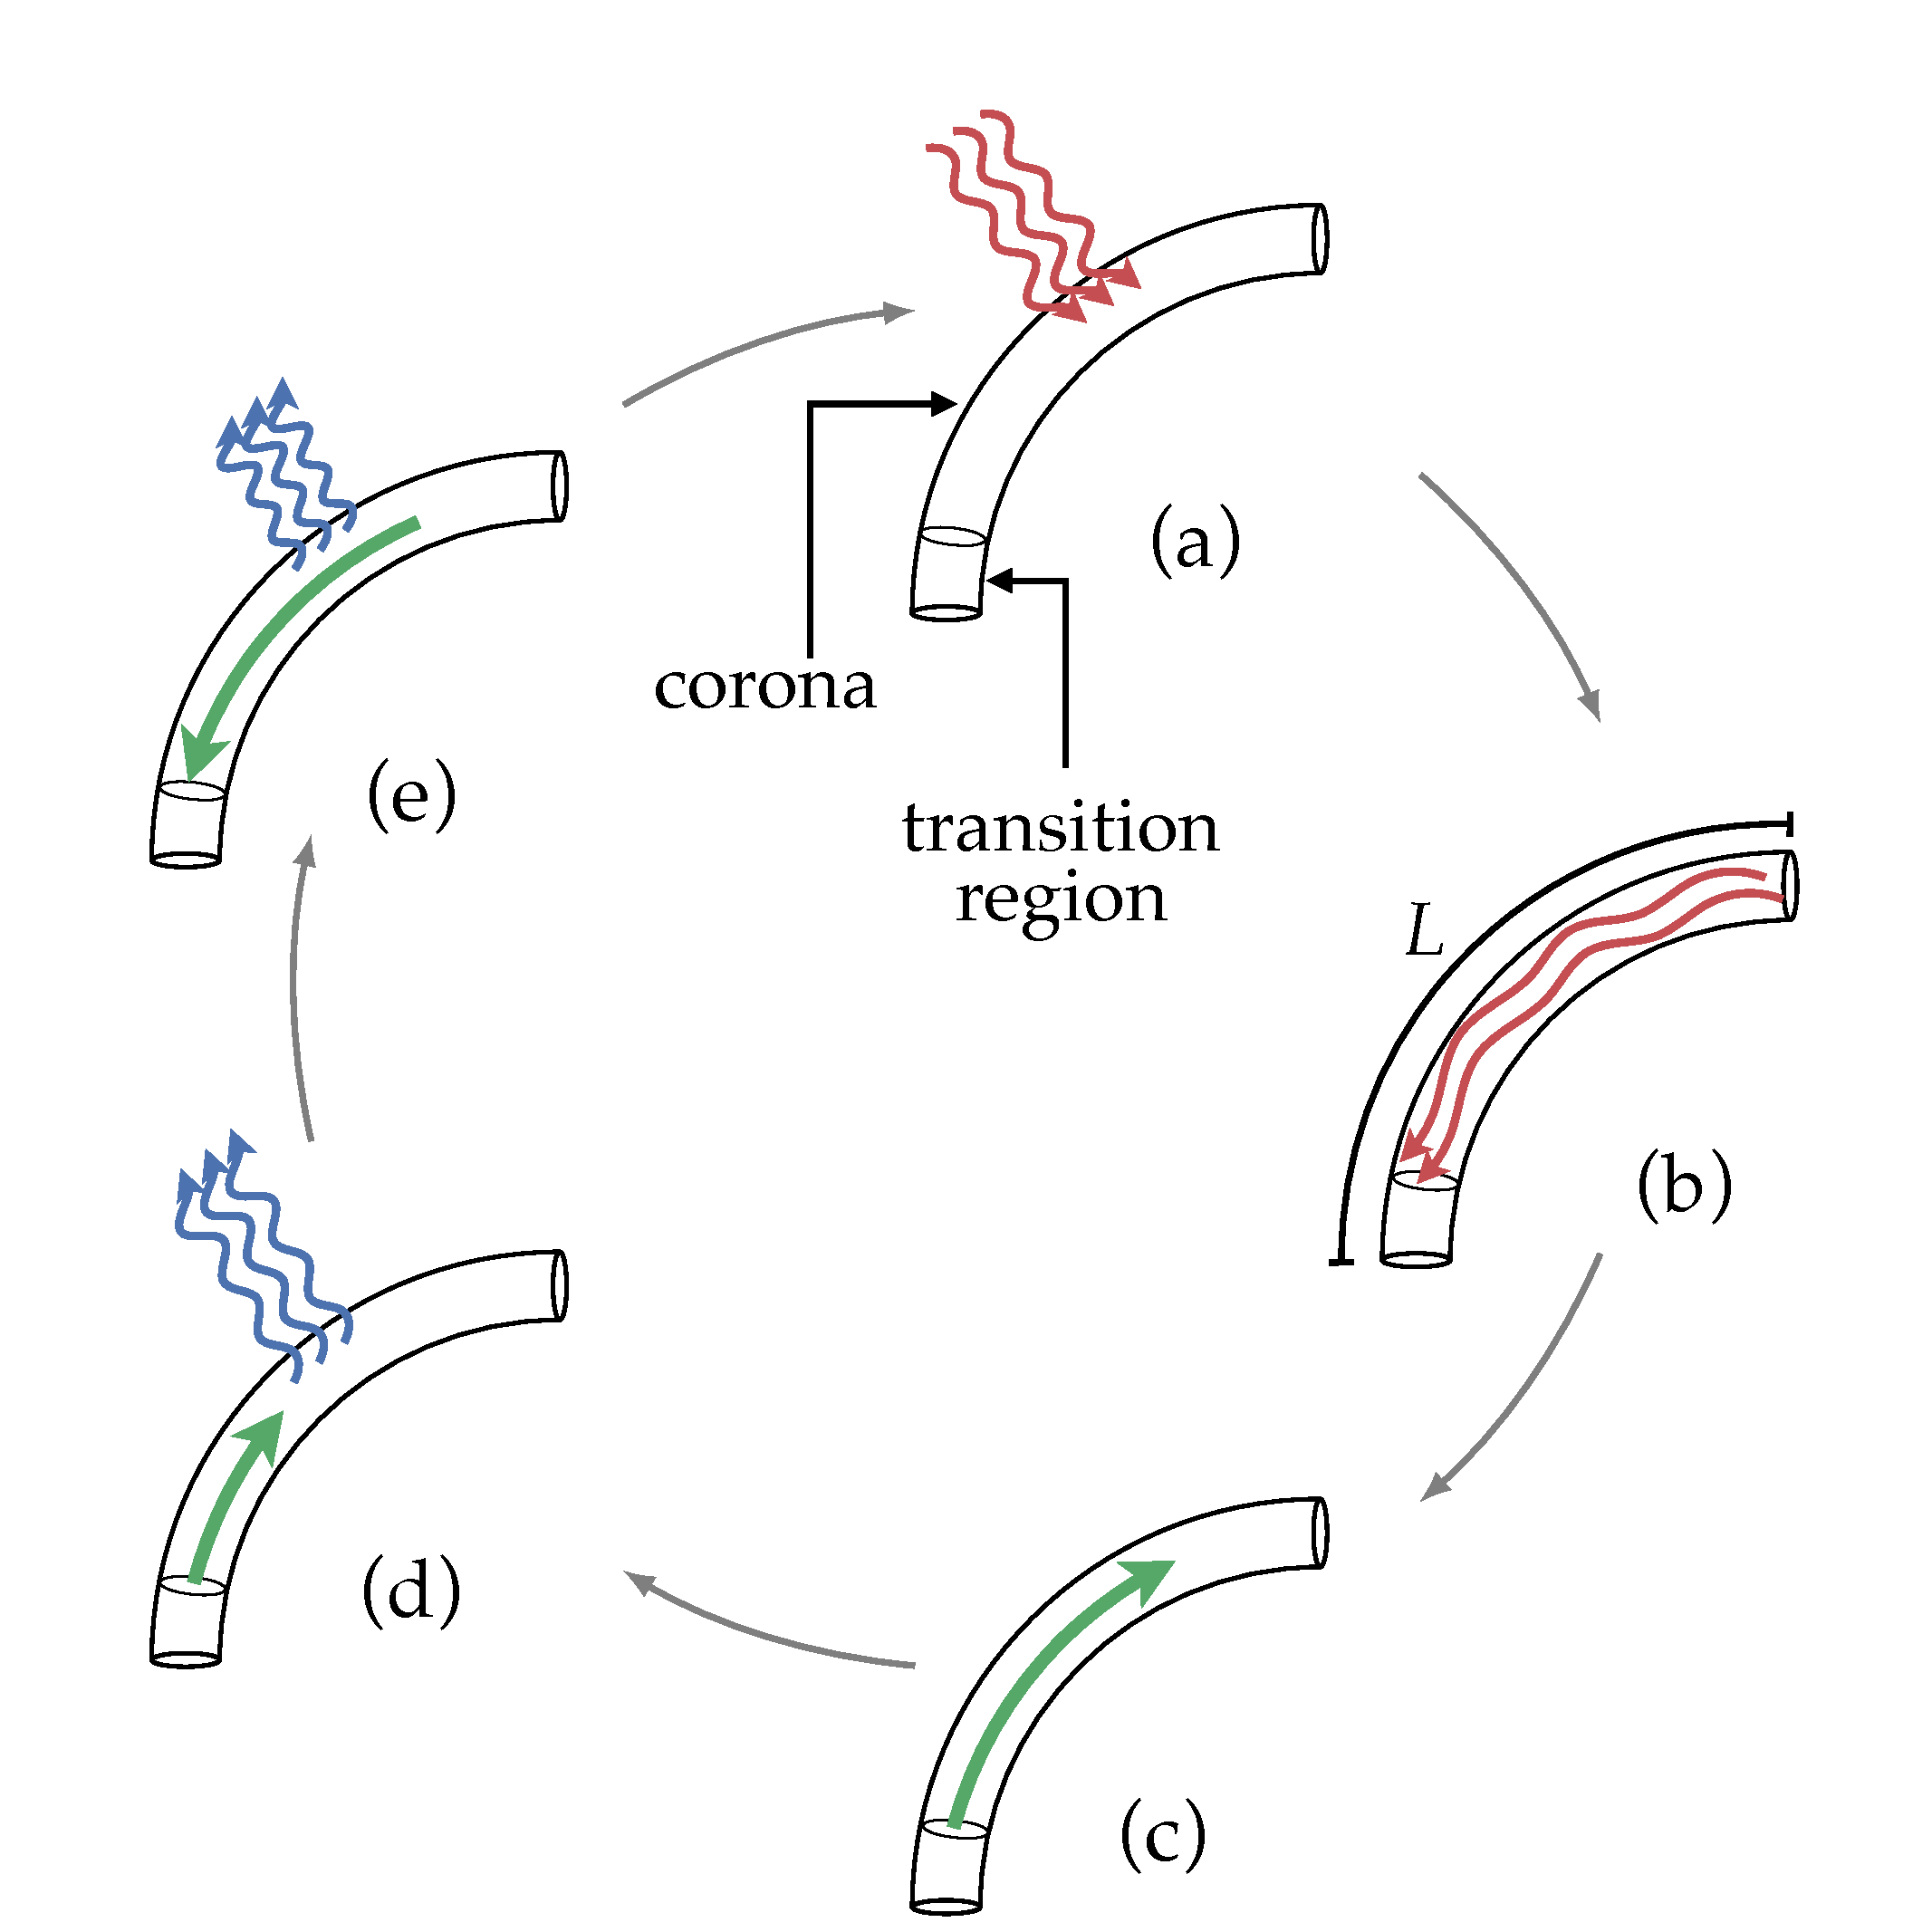
\includegraphics[width=0.65\textwidth]{chapter2/figures/heating-cooling-cycle-cartoon.pdf}
    \caption{A cartoon illustration of the heating and cooling cycle of an impulsively heated coronal loop. The loop has a half-length of $L$ and is assumed to be symmetric about the apex. The red arrows denote energy injected by heating (a) and energy transported by thermal conduction (b). The blue arrows denote energy lost by radiation (d and e). The thick green arrows indicate the bulk transport of material in the loop (c, d, and e). The black arrows denote the order in which the cycle proceeds.}
    \label{fig:heating-cooling-cycle-cartoon}
\end{figure}

If energy supplied by coronal heating cannot be balanced by radiation and thermal conduction in order to maintain hydrostatic equilibrium, the loop undergoes a cycle of heating, cooling, and draining according to the physics in \autoref{eq:hydrodynamic_mass}, \autoref{eq:hydrodynamic_momentum}, \autoref{eq:hydrodynamic_energy_e}, and \autoref{eq:hydrodynamic_energy_i}. This response of the coronal loop plasma to an impulsive release of energy is reasonably well-understood and has been studied extensively, both in the context of flares and nanoflares \citep[e.g.][]{antiochos_influence_1976,antiochos_evaporative_1978,cargill_implications_1994,cargill_cooling_1995,cargill_nanoflare_2004,bradshaw_cooling_2005,bradshaw_reinterpretation_2008,bradshaw_new_2010,bradshaw_cooling_2010}. \autoref{fig:heating-cooling-cycle-cartoon} shows a cartoon of the different phases of the heating, filling, cooling, and draining cycle of a coronal loop.

Consider a loop initially in hydrostatic equilibrium that is then (uniformly) heated sufficiently quickly such that radiation and thermal conduction do not have time to balance this energy input. For the sake of simplicity, I will assume the single-fluid approximation as given in \autoref{eq:hydrostatic_energy} and a semi-circular loop with half-length $L$ that is symmetric about the apex as shown in \autoref{fig:heating-cooling-cycle-cartoon}. This is illustrated in phase (a) of \autoref{fig:heating-cooling-cycle-cartoon}. This excess heat raises the temperature of the loop and sets up a strong heat flux toward the lower atmosphere because $F_c \propto -T^{5/2}\frac{\partial T}{\partial s}$ and $T$ monotonically increases with $s$ from the TR up to the apex. This is shown in phase (b). Once conduction is able to match the coronal heating rate, the plasma begins to cool.

Both radiation and conduction remove energy from corona and thus cool the plasma, but during this initial phase, conduction is more efficient. This is easily proved by considering the respective timescales of each of these processes. Following \citet{cargill_cooling_1995}, dropping all but the thermal conduction and radiative loss terms in \autoref{eq:hydrodynamic_energy} gives an apprximation of the conductive cooling time,
\begin{align}
    \frac{\partial}{\partial t}E \approx -\frac{\partial}{\partial s}F_c, \nonumber \\
    \frac{3k_BnT}{\tau_C} \sim \frac{\kappa_0 T^{7/2}}{L^2}, \nonumber \\
    \tau_C \sim \frac{3k_BL^2n}{\kappa_0T^{5/2}}, \label{eq:conductive_cooling_time}
\end{align} 
and the radiative cooling time,
\begin{align}
    \frac{\partial}{\partial t}E \approx -n^2\Lambda(T), \nonumber \\
    \frac{3k_BnT}{\tau_R} \sim n^2\chi T^\alpha, \nonumber \\
    \tau_R \sim \frac{3k_B}{\chi n T^{\alpha-1}}. \label{eq:radiative_cooling_time}
\end{align}
For $\alpha=-1/2$, $\tau_C \ll \tau_R$ for high temperatures and low densities such that conduction is more efficient than radiation at removing the excess energy in the corona. 

Because energy lost by radiation is proportional to $n^2$, the dense underlying chromosphere and TR are efficient at radiating away the energy conducted downward from the corona. However, if radiation cannot keep pace with the coronal conductive flux, this excess energy will heat the chromosphere and effectively destabilize the pressure balance in \autoref{eq:hydrostatic_pressure}. This increase in temperature causes chromospheric and TR \citep{bradshaw_influence_2013} material to expand into the corona and increase the coronal density. This process is illustrated in phase (c) of \autoref{fig:heating-cooling-cycle-cartoon} and is called chromospheric ablation\footnote{Historically, this process is referred to as chromospheric ``evaporation.'' However, this terminology is potentially misleading and ``ablation'' is a more accurate term.}. Note that this upflow of material provides energy to the corona via an enthalpy flux \citep{antiochos_evaporative_1978}.

As material fills the corona, $n$ increases and radiative cooling becomes more efficient. This further lowers the coronal temperature, weakens the downward conductive flux, and thus reduces chromospheric ablation. This is illustrated in panel (d). Once the corona has cooled sufficiently such that the downward conductive flux can be balanced by radiative losses in the TR, chromospheric ablation ceases. At this point, radiation has become just as efficient as thermal conduction such that $\tau_R\sim\tau_C$.

As the corona continues to cool, the ablated material can no longer support the upward pressure gradient and the plasma falls back down the loop due to gravity (see \autoref{eq:hydrostatic_pressure}). This is shown in phase (e) of \autoref{fig:heating-cooling-cycle-cartoon}. At this point, radiative cooling is much more efficient compared to conductive cooling such that $\tau_R\gg\tau_C$. However, \citep{bradshaw_cooling_2010} note that the resulting enthalpy flux out of the corona from the downflow of material also represents a significant and sometimes dominant loss mechanism during this radiative and enthalpy-driven cooling phase\footnote{While this phase of the loop evolution is often referrred to as only the ``radiative cooling phase,'' this nomenclature is incomplete as it neglects an important component of the energy budget.}. Furthermore, \citep{bradshaw_reinterpretation_2008,bradshaw_cooling_2010} show that this enthalpy flux is important in powering the TR against collapse due to runaway radiative cooling.

Provided the time-independent heating that initially supported the loop in hydrostatic equilibrium is still present, the loop will cool and drain until it reaches its equilibrium temperature and density. If the loop again undergoes some time-dependent heating, the cycle will start over. Note that the evolution of plasma is complicated if the loop is re-energized before the cooling and draining cycle is complete \citep[e.g.][or \autoref{sec:modeling-observables:heating}]{cargill_active_2014,barnes_inference_2016-1}.

\subsection{The HYDRAD Model}\label{sec:hydrad}

%Discuss HYDRAD in here, advantages, maybe a sample solution
% briefly discuss capabilities, numerical treatment

\subsection{The EBTEL Model}\label{sec:ebtel}

%Derive normal and two-fluid EBTEL equations, show examples

\subsubsection{Two-fluid Model}\label{sec:ebtel-two-fluid}

% Derivation of two-fluid model as given in second appendix of Barnes et al (2016a)
% details of numerical approach in ebtel++

Plugging in these expressions for $E_e$ and $E_i$ and using the assumptions of sub-sonic flows ($v<C_s$) and loops shorter than a gravitational scale height ($L<150$ Mm) as outlined in \citet{klimchuk_highly_2008}, the two-fluid field-aligned hydrodynamic energy equations can be written,
\begin{align}
    \frac{1}{\gamma - 1}\frac{\partial p_e}{\partial t} + \frac{\gamma}{\gamma - 1}\frac{\partial}{\partial s}(p_ev) &= v\frac{\partial p_e}{\partial s} - \frac{\partial F_{ce}}{\partial s} + \frac{1}{\gamma - 1}k_Bn\nu_{ei}(T_i-T_e) -n^2\Lambda(T_e)+Q_{e}, \label{eq:1denergy_e_simp} \\[0.5em]
    \frac{1}{\gamma - 1}\frac{\partial p_i}{\partial t} + \frac{\gamma}{\gamma - 1}\frac{\partial }{\partial s}(p_iv)&= -v\frac{\partial p_e}{\partial s} - \frac{\partial F_{ci}}{\partial s} + \frac{1}{\gamma - 1}k_Bn\nu_{ei}(T_e-T_i) + Q_{i}. \label{eq:1denergy_i_simp}
\end{align}
Notice that we have dropped the ion viscous and gravitational terms from  \autoref{eq:1denergy_i} as well as the kinetic energy term from \autoref{eq:ei_closure}. $Q_{e}$ and $Q_{i}$ represent the electron and ion heating terms, respectively. $F_{ce}$ and $F_{ci}$ are the electron and ion heat flux terms, respectively. In the case of Spitzer conduction, $\kappa_{0,e}=7.8\times10^{-7}$ and $\kappa_{0,i}=3.2\times10^{-8}$.

The analysis now follows that of \citet{klimchuk_highly_2008} and \citet{cargill_enthalpy-based_2012}. Assuming symmetry about the loop apex, we integrate \autoref{eq:1denergy_e_simp} and \autoref{eq:1denergy_i_simp} over the coronal loop half-length $L$,
\begin{align}
    \frac{L}{\gamma - 1}\frac{d \bar{p}_e}{dt} &= \frac{\gamma}{\gamma - 1}(p_ev)_0 + F_{ce,0} + \psi_C - \mathcal{R}_C + L\bar{Q}_{e},\label{eq:1denergy_e_C} \\[0.5em]
    \frac{L}{\gamma - 1}\frac{d \bar{p}_i}{dt} &= \frac{\gamma}{\gamma - 1}(p_iv)_0 + F_{ci,0} - \psi_C + L\bar{Q}_{i},\label{eq:1denergy_i_C}
\end{align}
where we have assumed the enthalpy flux and heat flux go to zero at the loop apex, $R_C=\int_C\mathrm{d}s\,n^2\Lambda(T_e)$ and,
\begin{equation}
    \psi_C=\int_C\mathrm{d}s\,v\frac{\partial p_e}{\partial s} + \int_C\mathrm{d}s\,\frac{k_B}{\gamma - 1}n\nu_{ei}(T_i - T_e).
\end{equation}

Similarly, integrating over the TR portion of the loop of thickness $\ell$, we obtain,
\begin{align}
    \frac{\gamma}{\gamma - 1}(p_ev)_0 &= - F_{ce,0} + \psi_{TR} - \mathcal{R}_{TR}, \label{eq:1denergy_e_TR} \\[0.5em]
    \frac{\gamma}{\gamma - 1}(p_iv)_0 &=  - F_{ci,0} - \psi_{TR}, \label{eq:1denergy_i_TR}
\end{align}
where several terms are neglected because $\ell\ll L$ \citep{klimchuk_highly_2008}. Additionally, we have assumed that the enthalpy flux and heat flux go to zero at the top of the chromosphere, $R_{TR}=\int_{TR}\mathrm{d}s\,n^2\Lambda(T_e)$ and
\begin{equation}
    \psi_{TR}=\int_{TR}\mathrm{d}s\,v\frac{\partial p_e}{\partial s} + \int_{TR}\mathrm{d}s\,\frac{k_B}{\gamma - 1}n\nu_{ei}(T_i - T_e).
\end{equation}
The second term in this expression is usually small, but is retained for completeness.  Plugging \autoref{eq:1denergy_e_TR} (\autoref{eq:1denergy_i_TR}) into \autoref{eq:1denergy_e_C} (\autoref{eq:1denergy_i_C}),
\begin{align}
    \frac{L}{\gamma - 1}\frac{d\bar{p}_e}{dt} =& \psi_{TR} + \psi_C -(\mathcal{R}_C + \mathcal{R}_{TR}) + L\bar{Q}_{e},\label{eq:0d_press_e_sub} \\[0.5em]
    \frac{L}{\gamma - 1}\frac{d\bar{p}_i}{dt} =& -(\psi_{C} + \psi_{TR}) +  L\bar{Q}_{i}.\label{eq:0d_press_i_sub}
\end{align}
Note that adding \autoref{eq:0d_press_e_sub} and \autoref{eq:0d_press_i_sub} gives the correct single-fluid EBTEL model (i.e. \autoref{eq:energy_0d}).

As in the single-fluid case, we find that the spatially-integrated coronal density evolution is described by,
\begin{equation}
    L\frac{d\bar{n}}{dt} = (nv)_0.
\end{equation}
Using \autoref{eq:1denergy_e_TR} and the equation of state for $p_e$, the above equation can be written as
\begin{align}
    (nv)_0 =& \frac{(p_ev)_0}{k_BT_{e,0}} = \frac{c_2(\gamma - 1)}{c_3\gamma k_B\bar{T}_e}(-F_{ce,0} - \mathcal{R}_{TR} + \psi_{TR}),\\
    L\frac{d\bar{n}}{dt} =& \frac{c_2(\gamma - 1)}{c_3\gamma k_B\bar{T}_e}(-F_{ce,0} - \mathcal{R}_{TR} + \psi_{TR}).\label{eq:0d_mass_sub}
\end{align}

To obtain \autoref{eq:press_e_0d_2fl}, \autoref{eq:press_i_0d_2fl}, and \autoref{eq:mass_0d_2fl}, we need to find expressions for $\psi_C$ and $\psi_{TR}$. Recall that $\psi_C$ and $\psi_{TR}$ are comprised of terms associated with the quasi-neutral electric field and temperature equilibration. The integral of the former can be considered as the gain or loss of energy associated with plasma motion through the net electric potential. Consider the first integral in the definition of $\psi_C$. Using integration by parts,
\begin{equation}
    \int_C\mathrm{d}s\,v\frac{\partial p_e}{\partial s} = (p_ev)\Big|^{``a"}_{``0"} - \int_C\mathrm{d}v\,p_e = -(p_ev)_0 - \int_C\mathrm{d}v\,p_e\approx -(p_ev)_0 -\bar{p}_e\int_C\mathrm{d}v = -(p_ev)_0 + \bar{p}_ev_0 \approx 0.
\end{equation}
Thus, we can express $\psi_C$ as
\begin{equation}
    \psi_C\approx\frac{k_BL}{\gamma -1}\bar{n}\nu_{ei}(\bar{T}_i - \bar{T}_e),
    \label{eq:psi_C}
\end{equation}
where $\nu_{ei}=\nu_{ei}(\bar{T}_e,\bar{n})$. To find an expression for $\psi_{TR}$, we first note that, using the equation of state for both the electrons and the ions and the quasi-neutrality condition ($n_e=n_i$),
\begin{equation}
    \frac{p_ev}{p_iv} = \frac{T_e}{T_i}.
\end{equation}
Evaluating this expression at the TR/corona interface (denoted by ``0''), plugging in \autoref{eq:1denergy_e_TR} and \autoref{eq:1denergy_i_TR},
\begin{equation}
    \frac{- F_{ce,0} + \psi_{TR} - \mathcal{R}_{TR}}{- F_{ci,0} - \psi_{TR}} = \xi,
\end{equation}
where $\xi\equiv T_{e,0}/T_{i,0}$. Solving for $\psi_{TR}$, we find,
\begin{equation}
    \psi_{TR} = \frac{1}{1+\xi}(F_{ce,0} + \mathcal{R}_{TR} - \xi F_{ci,0}).
    \label{eq:psi_TR}
\end{equation}

Plugging \autoref{eq:psi_C} and \autoref{eq:psi_TR} into \autoref{eq:0d_press_e_sub}, \autoref{eq:0d_press_i_sub}, and \autoref{eq:0d_mass_sub} gives us our set of two-fluid EBTEL equations as given in \autoref{eq:press_e_0d_2fl}, \autoref{eq:press_i_0d_2fl}, and \autoref{eq:mass_0d_2fl}. The prescription for $c_1$, $c_2$, and $c_3$ is the same as the single-fluid version of EBTEL. As discussed in \citet{cargill_enthalpy-based_2012}, these play little role in the early heating phase when two-fluid effects are important.

%% FIGURE HERE %%

Plugging \autoref{eq:psi_TR} into \autoref{eq:press_e_0d_2fl}, the electron energy evolution equation can be written,
\begin{equation}
    \frac{1}{\gamma -1}\frac{d\bar{p}_e}{dt} = \frac{1}{L(1+\xi)}F_{ce,0} - \frac{\xi}{L(1+\xi)}F_{ci,0} - \frac{\xi(c_1+1) + 1}{L(1+\xi)}\mathcal{R}_C + \frac{k_B}{\gamma-1}\bar{n}\nu_{ei}(\bar{T}_i-\bar{T}_e) + \bar{Q}_e,
    \label{eq:press_e_0d_2fl_breakdown}
\end{equation}
where the first two terms on the right-hand side represent the contributions from electron and ion thermal conduction, the third term represents losses from radiation, and the last two terms are as before. \autoref{fig:psi_tr_compare} shows the contribution of each term, with the exception of the heating term, $\bar{Q}_e$. As expected, (electron) thermal conduction dominates during the early heating and cooling phase and losses from radiation takeover in the late draining and cooling stage. Between these two phases, energy exchange between the two species is important to the evolution of the electron energy. $\psi_{TR}$, indicated by the black dotted line, is included to show its importance in the formation of the two-fluid EBTEL equations.

\subsubsection{Single-fluid Model}\label{sec:ebtel-single-fluid}

% Show how two-fluid equations simplify to single-fluid model
% point out that this was original model, developed by Klimchuk, Cargill, et al.

\subsubsection{Modifications to $c_1$ During the Conductive Cooling Phase}\label{sec:c1-correction}

In Section 3 of \citet{cargill_enthalpy-based_2012} we assumed that the parameter $c_1$ decreased from its equilibrium value at the time of maximum density, to that commensurate with radiative/enthalpy cooling as the loop drained. This was defined in terms of the ratio $n/n_{eq}$, where $n_{eq}$ was the loop density that would exist for the calculated temperature were the loop to be in static equilibrium \citep[Equation 17 of][]{cargill_enthalpy-based_2012}. In this radiative phase, $n > n_{eq}$. On the other hand, when $n < n_{eq}$, we assumed $c_1$ took on its equilibrium value, $c_{1,eq}$. Defining $\Delta\equiv(n_{\mathrm{EBTEL}} - n_{\mathrm{HYDRAD}})/n_{\mathrm{HYDRAD}}$, this gave $\Delta\lesssim0.2$, acceptable errors in the EBTEL value of $n$, as shown in the figures in \citet{cargill_enthalpy-based_2012}, in particular for the mild nanoflares we considered.

It is now clear that a modified description of $c_1$ for $n < n_{eq}$ is needed for many of the examples discussed in the present paper. Specifically, for intense heating events, the coronal density calculated by the version of EBTEL in \citet{cargill_enthalpy-based_2012} is unacceptably high when compared to results from the HYDRAD code. Quantitatively, we find $\Delta\gtrsim0.3$ at $n_{max}$. While this may seem to be reasonable for an aproximate model, the high EBTEL density is a systematic feature, and requires further investigation.

Examination of the HYDRAD results shows that EBTEL significantly underestimates the TR radiative losses during the heating and conductive cooling phases. At this time, the loop is under-dense \citep[e.g.][]{cargill_nanoflare_2004}, so that an excess of the conducted energy goes into evaporating TR material. We have modified $c_1$ as follows for $n < n_{eq}$,
\begin{equation}
    c_1 = \frac{2c_{1,eq} + c_{1,cond}((n_{eq}/n)^2-1)}{1+(n_{eq}/n)^2},
    \label{eq:c1_mod}
\end{equation}
as a direct analogy to Eq. 18 of \citet{cargill_enthalpy-based_2012}. In the early phases of an event, $n \ll n_{eq}$, so that $c_1 \approx c_{1,cond}$. When $n = n_{eq}$, $c_1 = c_{1,eq}$. After some experimentation, we have settled on a choice of $c_{1,cond} = 6$ since that gives reasonable agreement between EBTEL and HYDRAD. There is no impact on the solution for $n > n_{eq}$.

\autoref{tab:table_c1_compare} shows a set of runs we have carried out to compare the results from HYDRAD and EBTEL with $c_1=c_{1,eq}=2$ (fifth column) and with $c_1$ given by \autoref{eq:c1_mod} (sixth column), when $n<n_{eq}$. We find that using the modification in \autoref{eq:c1_mod} gives, for the more intense heating cases with $\tau\ge200$ s, $\Delta\sim0.1$ at $n_{max}$. For the more gentle heating profiles of \citet{cargill_enthalpy-based_2012} and \citet{bradshaw_influence_2013} (i.e. rows 3, 4, 6, and 8 of \autoref{tab:table_c1_compare}), we continue to find $\Delta\lesssim0.2$, confirming that the modification proposed here is applicable to a wide range of heating scenarios. For short, intense pulses like the $\tau=20,40$ s cases addressed in this paper, we still find $\Delta>0.2$. The limitations of such cases are addressed in \autoref{hot-plasma:subsubsec:hydrad_comparison_sf}.

% RESULTS TABLE HERE %

\autoref{eq:c1_mod} is motivated by simplicity while including the essential physics. Alternative, more complex determinations of $c_1$ have been considered, but involve limitations on how EBTEL can be used both now and in the future.

\nomenclature[a-ti]{$T_i$}{ion temperature}
\nomenclature[a-me]{$m_e$}{electron mass}
\nomenclature[a-mi]{$m_i$}{ion mass}
\nomenclature[a-gsol]{$g_\solar$}{gravitational acceleration at the solar surface}